% \section{Introduction}
We analyse the execution of multiple models on the GrAICore.
We assume that each of these models fit on the GrAICore individually.
% We will be looking at the execution of multiple models on the GrAICore.
% We assume that each of these models fit on the GrAICore individually.

\section{Bandwidth analysis}

To determine the required write bandwidth for configuring a model, we need the following parameters:
\begin{itemize}
    \item The input frame rate
    \item The amount of bytes to be written
    \item The frame processing latency
\end{itemize}

The amount of time we have to configure the GrAICore is depend on the input frame rate and frame processing latency.
For example, for an input frame rate of \SI{60}{FPS}, we have a period of \SI{16.7}{ms} between every two frames.
Suppose we want to process every new incoming frame with a new model, all with a frame processing latency of \SI{5}{ms}. 
Due to the frame processing latency, we only have a time budget of \SI{11.7}{ms} to reconfigure the GrAICore with the next model.

\begin{figure}[htbp]
    \centering
    \begin{tikzpicture}[scale=0.5]
    \draw[] (6,0) -- (24,0);
    \draw[dashed, ->] (24,0) -- (25,0);
    \draw (6,0.5) -- (6,-0.5) node[below] {$0$};
    \draw (12,0.5) -- (12,-0.5) node[below] {$T$};
    \draw (18,0.5) -- (18,-0.5) node[below] {$2T$};
    \draw (24,0.5) -- (24,-0.5) node[below] {$3T$};
    % \draw (6,0.5) -- (6,-0.5) node[below] {$t_{0}$};
    % \draw (12,0.5) -- (12,-0.5) node[below] {$t_{1}$};
    % \draw (18,0.5) -- (18,-0.5) node[below] {$t_{2}$};
    % \draw (24,0.5) -- (24,-0.5) node[below] {$t_{3}$};

    \draw [pattern=north east lines, pattern color=gray, line width = 1pt, very thick] ($(6,0)$) rectangle ++($(1.5,1)$) node[midway] {$p_A$};
    \draw [pattern=north west lines, pattern color=gray, line width = 1pt, very thick] ($(7.5,0)$) rectangle ++($(3,1)$) node[midway] {$c_B$};
    % \draw [decorate,decoration={brace,amplitude=6pt}]($(6,1.5)$) -- ++($(1.5,0)$) node [black,midway,above=6pt] {\tiny L};
    
    \draw [pattern=north east lines, pattern color=gray, line width = 1pt, very thick] ($(12,0)$) rectangle ++($(1.5,1)$) node[midway] {$p_B$};
    \draw [pattern=north west lines, pattern color=gray, line width = 1pt, very thick] ($(13.5,0)$) rectangle ++($(3,1)$) node[midway] {$c_C$};
    % \draw [decorate,decoration={brace,amplitude=6pt}]($(12,1.5)$) -- ++($(1.5,0)$) node [black,midway,above=6pt] {\tiny L};
    
    \draw [pattern=north east lines, pattern color=gray, line width = 1pt, very thick] ($(18,0)$) rectangle ++($(1.5,1)$) node[midway] {$p_C$};
    \draw [pattern=north west lines, pattern color=gray, line width = 1pt, very thick] ($(19.5,0)$) rectangle ++($(3,1)$) node[midway] {$c_D$};
    % \draw [decorate,decoration={brace,amplitude=6pt}]($(18,1.5)$) -- ++($(1.5,0)$) node [black,midway,above=6pt] {\tiny L};
\end{tikzpicture}

    \caption{TODO}
    \label{fig:reconfig_time_line_ex3}
\end{figure}

We calculate the required bandwidth for configuring model $m$ with \cref{eq:multiple_models_bandwidth}.
\begin{equation}
    B_m = \frac{D_m}{\frac{1}{f} - L_m}
    \label{eq:multiple_models_bandwidth}
\end{equation}

\begin{eqexpl}[15mm]
    \item{$B_m$} required bandwidth for writing model $m$
    \item{$D_m$} amount of bytes to write for model $m$
    \item{$f$} input frame rate
    \item{$L_m$} frame processing latency for model $m$
\end{eqexpl}

In the worst-case scenario, we have configure the GrAICore with a model requiring to write the total capacity of the GrAICore (\SI{36}{MiB}).
We require a minimum write bandwidth of $\SI{3086}{MiB/s}$\footnote{$\frac{\SI{36}{MiB}}{\frac{1}{\SI{60}{FPS}} - \SI{5}{ms}} \approx \SI{3086}{MiB/s}$} for $\SI{60}{FPS}$.
Note that this bandwidth number does not include any overhead induced by communication protocols. Therefore, in practice, the required minimum bandwidth is higher. 

\Cref{fig:frame_rate_versus_time_budget} shows that an increase in frame rate decreases the available time budget for reconfiguration.
\Cref{tab:common_fps} shows a list of common video frame rates with their associated reconfiguration time budget.
A frame rate with zero or negative time budget means that the GrAICore cannot be reconfigured seamlessly for a video with the corresponding frame rate.
Exceeding this time budget results into a delayed output which is undesirable since it negatively affects the user experience.
At a frame rate of $\SI{200}{FPS}$, the time budget is exactly zero, indicating that this represents the tight upper bound.
% \begin{equation}
%     B = f^{-1} - \SI{5}{ms}
% \end{equation}

% \begin{figure}[htbp]
%     \centering
%     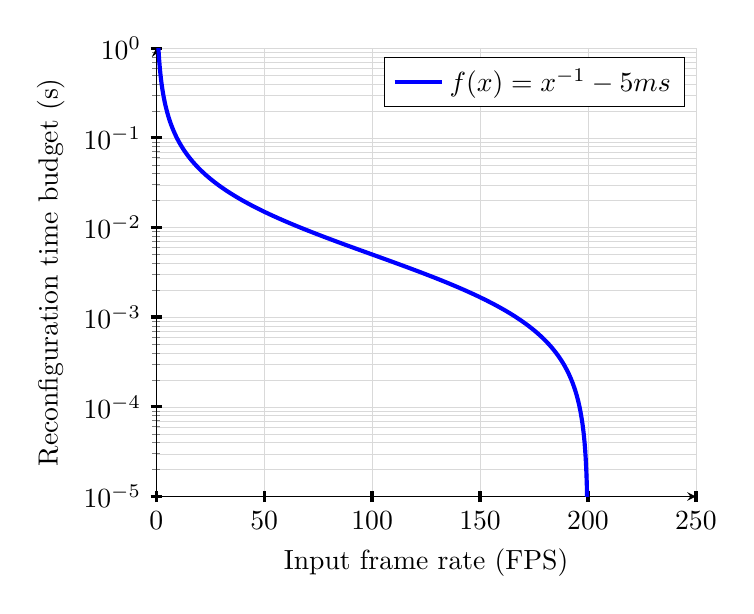
\begin{tikzpicture}
\begin{semilogyaxis}[
    xmin=0, xmax=250,
    ymin=0.00001, ymax=1,
    axis lines = left,
    xlabel = {Input frame rate (FPS)},
    ylabel = {Reconfiguration time budget (s)},
    ymajorgrids=true,
    grid=both,
    % grid style=dashed,
    grid style={line width=.1pt, draw=gray!30},
    every major tick/.append style={very thick, major tick length=4pt, black},
]

% 16 bits
\addplot[
    domain=0:250, 
    samples=1000, 
    color=blue,
    line width=1.5pt
]
{1/x - 0.005};
% \addlegendentry{$B(f) = f^{-1} - \SI{5}{ms}$}
\addlegendentry{$f(x) = x^{-1}  - \SI{5}{ms}$}
\end{semilogyaxis}
\end{tikzpicture}

%     \caption{An increase in frame rate lowers the reconfiguration time budget}
%     \label{fig:fps_vs_budget}
% \end{figure}


\begin{figure}[htbp]
    \centering
    \begin{subfigure}[b]{0.48\textwidth}
        \begin{adjustbox}{width=\linewidth}
        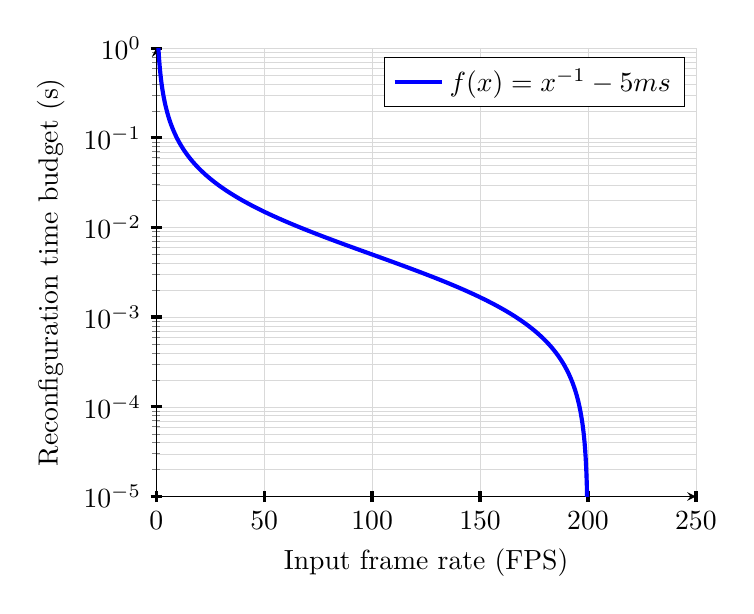
\begin{tikzpicture}
\begin{semilogyaxis}[
    xmin=0, xmax=250,
    ymin=0.00001, ymax=1,
    axis lines = left,
    xlabel = {Input frame rate (FPS)},
    ylabel = {Reconfiguration time budget (s)},
    ymajorgrids=true,
    grid=both,
    % grid style=dashed,
    grid style={line width=.1pt, draw=gray!30},
    every major tick/.append style={very thick, major tick length=4pt, black},
]

% 16 bits
\addplot[
    domain=0:250, 
    samples=1000, 
    color=blue,
    line width=1.5pt
]
{1/x - 0.005};
% \addlegendentry{$B(f) = f^{-1} - \SI{5}{ms}$}
\addlegendentry{$f(x) = x^{-1}  - \SI{5}{ms}$}
\end{semilogyaxis}
\end{tikzpicture}

        \end{adjustbox}
        \caption{An increase in frame rate lowers the reconfiguration time budget}
        \label{}
    \end{subfigure}
    \hfill
    \begin{subfigure}[b]{0.48\textwidth}
        \begin{tabular}{@{}ll@{}}
        \toprule
        Frame rate (FPS) & Reconf. budget (ms) \\ \midrule
        15               & 61.7                \\
        24               & 36.7                \\
        30               & 28.3                \\
        60               & 11.7                \\
        120              & 3.3                 \\
        200              & 0.0                 \\
        240              & -0.8                \\ \bottomrule
        \end{tabular}
        \caption{Reconfiguration time budget for different common video frame rates}
        \label{tab:common_fps}
    \end{subfigure}
    \caption[]{Input frame rate versus reconfiguration time budget}
    \label{fig:frame_rate_versus_time_budget}
\end{figure}

If we have a set of different models we want to switch between, we need to be able to reach the highest required bandwidth:
\begin{equation*}
    B = \max\{\,m \in M \mid B_m \,\} 
\end{equation*}